\documentclass[manuscript]{acmart}

%% Rights and Conference Management Configuration for Course Submission
\setcopyright{none}
\settopmatter{printacmref=false}
\renewcommand\footnotetextcopyrightpermission{}
\pagestyle{plain}

\acmJournal{CSUR}

%% Essential Packages
\usepackage{booktabs}
\usepackage{amsmath}
\usepackage{amssymb}
\usepackage{microtype}
\usepackage{tabularx}
\usepackage{array}
\usepackage{tikz}
\usetikzlibrary{arrows.meta,positioning,shapes.geometric,fit,calc}

\begin{document}

\title{Context-Window Degradation and Its Impact on Long-Document Research Synthesis: A Survey}

\author{Pranav Kumar Gupta}
\authornote{Roll No.: MHM2026012. Course assignment manuscript on AI-assisted scientific writing.}
\affiliation{%
  \institution{Indian Institute of Information Technology Allahabad}
  \city{Prayagraj}
  \state{Uttar Pradesh}
  \country{India}
}

\begin{abstract}
Large Language Models (LLMs) have achieved substantial increases in nominal context windows, scaling from thousands to millions of tokens. This expansion has generated widespread optimism for automating comprehensive scientific synthesis, legal brief examination, and long-range repository analysis. However, a growing body of empirical literature reveals that architectural context limits do not equal effective reasoning capacity. This survey systematically investigates \emph{context-window degradation}---the performance deterioration observed as sequence lengths expand. We review the mathematical and structural causes of degradation, including attention dilution, primacy and recency biases, and positional out-of-distribution shifts. We examine diagnostic benchmarks ranging from lexical Needle-In-A-Haystack (NIAH) probes to semantic evaluation suites like NoLiMa, alongside the formulation of the Maximum Effective Context Window (MECW). Furthermore, we review compensatory mechanisms, including Retrieval-Augmented Generation (RAG), long-chunk frameworks (LongRAG), dynamic context selection (Adaptive-$k$), and architectural position-embedding adaptations (RoPE, ALiBi, Position Interpolation). Finally, we provide structured comparative matrices of reviewed paradigms, analyze multi-dimensional system trade-offs, and outline key open research problems required to realize reliable long-document synthesis.
\end{abstract}

\begin{CCSXML}
<ccs2012>
   <concept>
       <concept_id>10010147.10010178.10010179</concept_id>
       <concept_desc>Computing methodologies~Natural language processing</concept_desc>
       <concept_significance>500</concept_significance>
       </concept>
   <concept>
       <concept_id>10002951.10003317.10003347</concept_id>
       <concept_desc>Information systems~Retrieval models and ranking</concept_desc>
       <concept_significance>400</concept_significance>
       </concept>
   <concept>
       <concept_id>10010147.10010257.10010293.10010294</concept_id>
       <concept_desc>Computing methodologies~Neural networks</concept_desc>
       <concept_significance>300</concept_significance>
       </concept>
 </ccs2012>
\end{CCSXML}

\ccsdesc[500]{Computing methodologies~Natural language processing}
\ccsdesc[400]{Information systems~Retrieval models and ranking}
\ccsdesc[300]{Computing methodologies~Neural networks}

\keywords{Context-Window Degradation, Long-Context Language Models, Lost in the Middle, Maximum Effective Context Window, Retrieval-Augmented Generation, Needle in a Haystack, Literature Survey}

\maketitle

\section{Introduction}\label{sec:intro}
The expansion of input context windows in transformer-based Large Language Models (LLMs) represents a central thrust of modern natural language processing. Successive iterations of frontier and open-weight architectures have expanded nominal input horizons from 2,048 tokens in original foundation models to hundreds of thousands or millions of tokens \cite{vaswani2017attention,su2024roformer,chen2023interpolation}. In theory, these multi-million-token windows enable the end-to-end ingestion and synthesis of entire literature corpuses, multi-volume legal proceedings, comprehensive technical documentation, and long-range historical archives in a single forward pass.

Despite these marketed capacities, empirical evaluations identify a stark divergence between \emph{nominal context capacity} and \emph{effective utilization} \cite{liu2024lost,paulsen2025mecw}. When models are tasked with long-document synthesis---such as reconciling conflicting empirical findings across distinct publications, tracking multi-hop causal chains, or extracting thematic arguments---their performance exhibits severe degradation. Rather than operating uniformly across the available sequence, models suffer from selective inattention, hallucinated synthesis, attribution errors, and acute sensitivity to the structural placement of evidence \cite{liu2024lost,dai2024deniahl}.

This phenomenon is broadly termed \emph{context-window degradation}. Understanding its root causes requires examining the mechanics of the self-attention operation \cite{vaswani2017attention}, position-encoding decay \cite{press2022alibi,su2024roformer}, and training-data distribution artifacts. The practical impact on scientific research synthesis is acute: research synthesis demands high recall across dense, inter-dependent literature where critical caveats, methodologies, and quantitative metrics are distributed throughout the text rather than concentrated in introductory or concluding summaries.

\paragraph{Scope and Contributions}
This survey provides a structured, scholarly analysis of context-window degradation and the paradigms proposed to address it. We deliberately frame this work as a literature review of external research. Specifically, our contributions include:
\begin{enumerate}
    \item A review of the theoretical and architectural mechanisms governing context degradation, including attention dilution, positional bias, and representation drift.
    \item An examination of diagnostic frameworks, establishing the divergence between surface-level lexical recall (e.g., standard Needle-in-a-Haystack tests) and semantic reasoning across long contexts.
    \item A technical classification and comparative evaluation of mitigation paradigms, contrasting full-context ingestion, standard retrieval-augmented pipelines, long-chunk hybrid systems, and adaptive context selectors.
    \item Conceptual formalisms for computational complexity scaling and effective context retention, paired with a multi-dimensional system trade-off matrix.
    \item A roadmap of open research gaps in loss formulation, memory architectures, and benchmark rigor.
\end{enumerate}

\section{Review Methodology}\label{sec:methodology}
To structure this survey, we followed a systematic four-phase review workflow, illustrated in Figure~\ref{fig:methodology}.

\begin{figure}[htbp]
\centering
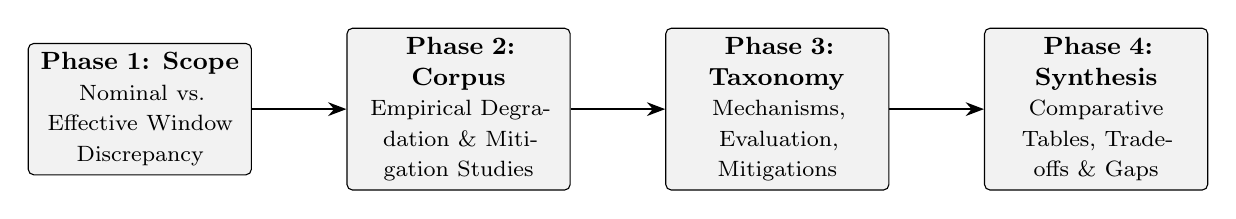
\begin{tikzpicture}[
    node distance=0.85cm and 1.2cm,
    every node/.style={font=\small},
    block/.style={rectangle, draw=black, rounded corners=2pt, fill=gray!10, text width=2.6cm, align=center, minimum height=1.1cm},
    arrow/.style={-Stealth, thick, draw=black}
]
    \node [block] (p1) {\textbf{Phase 1: Scope}\\\footnotesize Nominal vs. Effective Window Discrepancy};
    \node [block, right=of p1] (p2) {\textbf{Phase 2: Corpus}\\\footnotesize Empirical Degradation \& Mitigation Studies};
    \node [block, right=of p2] (p3) {\textbf{Phase 3: Taxonomy}\\\footnotesize Mechanisms, Evaluation, Mitigations};
    \node [block, right=of p3] (p4) {\textbf{Phase 4: Synthesis}\\\footnotesize Comparative Tables, Trade-offs \& Gaps};

    \draw [arrow] (p1) -- (p2);
    \draw [arrow] (p2) -- (p3);
    \draw [arrow] (p3) -- (p4);
\end{tikzpicture}
\caption{Systematic literature review workflow, illustrating the progression from scope definition to taxonomic classification and comparative synthesis.}
\label{fig:methodology}
\end{figure}

The review scope was bounded by studies examining transformer context degradation, long-document question answering, and retrieval augmentation published or archived between 2017 and 2026. Studies were grouped according to the taxonomy presented in Figure~\ref{fig:taxonomy}.

\begin{figure*}[htbp]
\centering
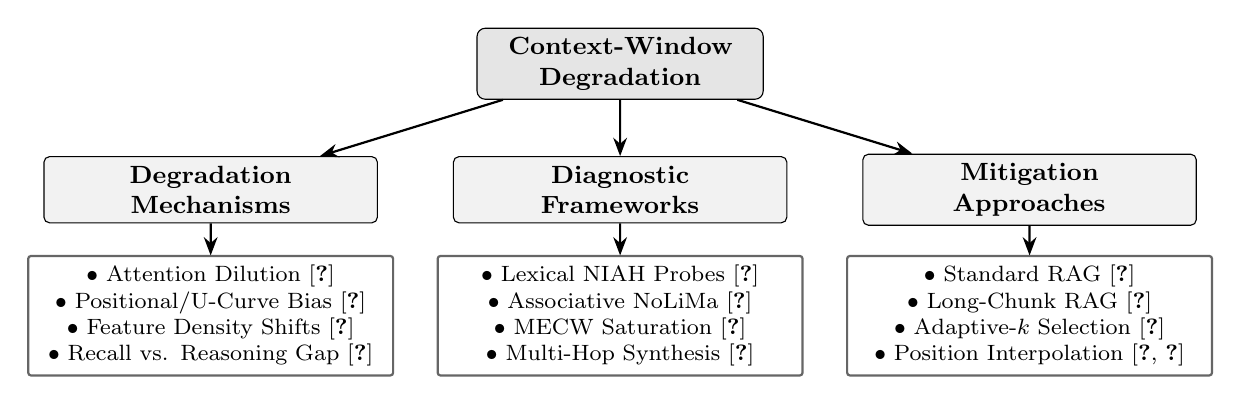
\begin{tikzpicture}[
    level distance=1.6cm,
    sibling distance=5.2cm,
    edge from parent/.style={draw=black, -Stealth, thick},
    every node/.style={font=\small, align=center},
    root/.style={rectangle, draw=black, fill=gray!20, rounded corners=3pt, text width=3.4cm, minimum height=0.9cm, font=\small\bfseries},
    category/.style={rectangle, draw=black, fill=gray!10, rounded corners=2pt, text width=4.0cm, minimum height=0.8cm, font=\small\bfseries},
    leaf/.style={rectangle, draw=black!60, fill=white, rounded corners=1pt, text width=4.4cm, minimum height=1.3cm, font=\footnotesize}
]
\node [root] {Context-Window\\Degradation}
    child {
        node [category] {Degradation\\Mechanisms}
        child {
            node [leaf] {
                $\bullet$ Attention Dilution~\cite{vaswani2017attention}\\
                $\bullet$ Positional/U-Curve Bias~\cite{liu2024lost}\\
                $\bullet$ Feature Density Shifts~\cite{dai2024deniahl}\\
                $\bullet$ Recall vs. Reasoning Gap~\cite{paulsen2025mecw}
            }
        }
    }
    child {
        node [category] {Diagnostic\\Frameworks}
        child {
            node [leaf] {
                $\bullet$ Lexical NIAH Probes~\cite{dai2024deniahl}\\
                $\bullet$ Associative NoLiMa~\cite{modarressi2025nolima}\\
                $\bullet$ MECW Saturation~\cite{paulsen2025mecw}\\
                $\bullet$ Multi-Hop Synthesis~\cite{zhao2024longrag}
            }
        }
    }
    child {
        node [category] {Mitigation\\Approaches}
        child {
            node [leaf] {
                $\bullet$ Standard RAG~\cite{lewis2020rag}\\
                $\bullet$ Long-Chunk RAG~\cite{zhao2024longrag}\\
                $\bullet$ Adaptive-$k$ Selection~\cite{taguchi2025adaptivek}\\
                $\bullet$ Position Interpolation~\cite{chen2023interpolation,press2022alibi}
            }
        }
    };
\end{tikzpicture}
\caption{Taxonomy of context-window degradation: mechanisms, diagnostic evaluation frameworks, and mitigation paradigms.}
\label{fig:taxonomy}
\end{figure*}

\section{Mechanisms of Context Degradation}\label{sec:mechanisms}
Context degradation is not an anomalous artifact of specific model checkpoints, but an emergent consequence of standard self-attention architectures and optimization objectives.

\subsection{Mathematical Foundations of Attention Dilution}
In standard scaled dot-product attention \cite{vaswani2017attention}, input representations are projected into queries $Q \in \mathbb{R}^{N \times d_k}$, keys $K \in \mathbb{R}^{N \times d_k}$, and values $V \in \mathbb{R}^{N \times d_v}$, where $N$ denotes sequence length and $d_k$ is key dimensionality. The attention weights are evaluated as:
\begin{equation}
    \mathrm{Attention}(Q, K, V) = \mathrm{softmax}\left(\frac{QK^T}{\sqrt{d_k}}\right)V.
    \label{eq:attention}
\end{equation}
The computational and memory requirements of standard dense attention scale quadratically with context length $N$:
\begin{equation}
    \mathcal{C}_{\mathrm{attn}}(N) = \mathcal{O}(N^2 \cdot d_k) \quad \text{and} \quad \mathcal{M}_{\mathrm{attn}}(N) = \mathcal{O}(N^2 + N \cdot d_v).
    \label{eq:complexity}
\end{equation}

Beyond computational constraints \eqref{eq:complexity}, expanding sequence length $N$ imposes representational challenges. Because the softmax function normalizes attention scores across all $N$ tokens, the probability mass allocated to each token necessarily decreases in the presence of extensive distractor text. As $N$ reaches tens or hundreds of thousands of tokens, entropy across the distribution increases, dampening key activation signals and causing representational dilution.

\subsection{Primacy and Recency Positional Bias}
A prominent manifestation of context degradation is the ``lost in the middle'' phenomenon identified by Liu et al.~\cite{liu2024lost}. When language models are presented with multi-document prompts containing target information at varying relative depths, retrieval performance follows an asymmetric U-shaped curve. 

\begin{figure}[htbp]
\centering
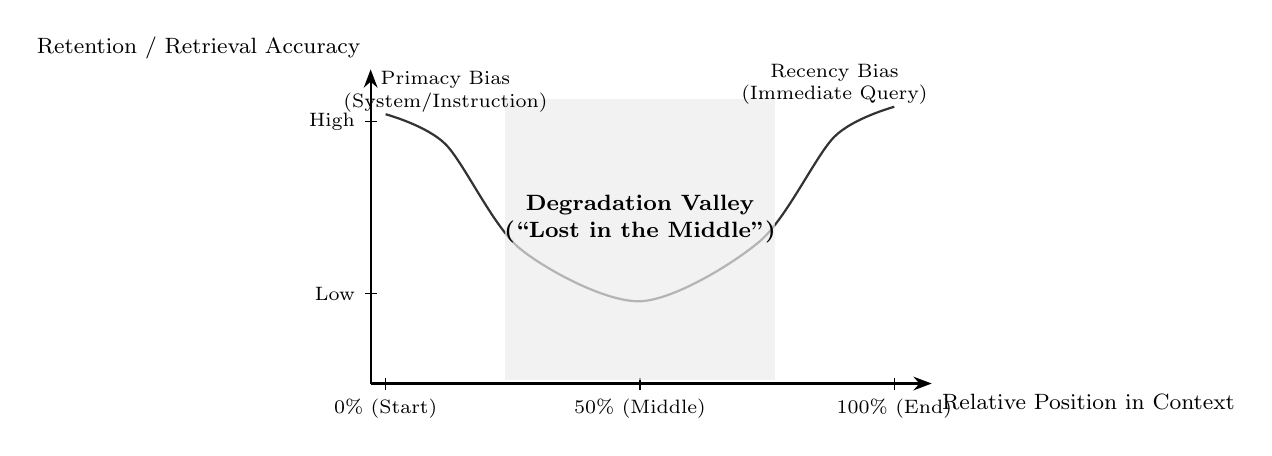
\begin{tikzpicture}[scale=0.95]
    % Axes
    \draw[-Stealth, thick] (0,0) -- (7.5,0) node[below right, font=\footnotesize] {Relative Position in Context};
    \draw[-Stealth, thick] (0,0) -- (0,4.2) node[above left, font=\footnotesize] {Retention / Retrieval Accuracy};

    % Ticks and labels
    \draw (0.2,0.08) -- (0.2,-0.08) node[below, font=\scriptsize] {0\% (Start)};
    \draw (3.6,0.08) -- (3.6,-0.08) node[below, font=\scriptsize] {50\% (Middle)};
    \draw (7.0,0.08) -- (7.0,-0.08) node[below, font=\scriptsize] {100\% (End)};

    \draw (0.08,3.5) -- (-0.08,3.5) node[left, font=\scriptsize] {High};
    \draw (0.08,1.2) -- (-0.08,1.2) node[left, font=\scriptsize] {Low};

    % U-Curve (Conceptual)
    \draw[thick, black!80, smooth] plot coordinates {
        (0.2, 3.6)
        (1.0, 3.2)
        (2.0, 1.8)
        (3.6, 1.1)
        (5.2, 1.9)
        (6.2, 3.3)
        (7.0, 3.7)
    };

    % Shaded degradation valley
    \fill[gray!15, opacity=0.7] (1.8,0.05) rectangle (5.4,3.8);
    \node[font=\footnotesize\bfseries, align=center] at (3.6,2.2) {Degradation Valley\\(``Lost in the Middle'')};

    % Labels for Primacy and Recency
    \node[font=\scriptsize, align=center] at (1.0,3.9) {Primacy Bias\\(System/Instruction)};
    \node[font=\scriptsize, align=center] at (6.2,4.0) {Recency Bias\\(Immediate Query)};
\end{tikzpicture}
\caption{Conceptual schematic of the U-shaped positional effect observed in multi-document retrieval tasks. Performance peaks at the prompt extremities and degrades substantially across intermediate positions. Note: This plot is an illustrative conceptual framing of literature findings \cite{liu2024lost}, not empirical laboratory measurements.}
\label{fig:lost_in_middle}
\end{figure}

As conceptualized in Figure~\ref{fig:lost_in_middle}, accuracy peaks when critical facts are placed within the opening tokens (primacy bias) or closing tokens (recency bias), but plummets when target passages reside in the central $20\%\text{--}80\%$ of the context. This pattern stems from optimization priors: pre-training corpora (e.g., articles, books, code repositories) concentrate architectural instructions and high-level summaries at document headers, while instruction-tuning reinforces reliance on trailing user queries. Intermediate context is thus treated with reduced effective attention weight.

\section{Evaluation Paradigms and the Effective Window}\label{sec:eval_frameworks}

\subsection{Needle-In-A-Haystack and In-Context Feature Sensitivity}
The primary sanity check for long-context models has been the synthetic Needle-in-a-Haystack (NIAH) benchmark. In this protocol, a distinct factual assertion (the ``needle'') is inserted at an arbitrary depth within unrelated filler text (the ``haystack''). While production models frequently advertise near-$100\%$ retrieval on standard NIAH tests, Dai et al.~\cite{dai2024deniahl} demonstrated through the DENIAHL benchmark that standard NIAH results mask severe fragility. In-context variables---such as semantic overlap between needle and filler, lexical density, distractor frequency, and syntactic complexity---substantially reduce retrieval fidelity. When distractor passages exhibit high topical similarity to the query, attention sinks route probability mass away from the target needle.

\subsection{Beyond Literal Matching: Semantic Reasoning Gaps}
A critical limitation of conventional benchmarks is their reliance on verbatim keyword matching. In realistic research synthesis, answers are rarely stored as isolated sentences; rather, synthesis requires semantic cross-referencing and deductive inference. Modarressi et al.~\cite{modarressi2025nolima} introduced NoLiMa to evaluate non-literal long-context understanding. Their findings revealed that while state-of-the-art models maintain high recall on literal extraction at sequence lengths up to 32,000 tokens, their capacity to infer latent associations drops below $50\%$ over identical context spans.

\subsection{The Maximum Effective Context Window (MECW)}
To resolve the discrepancy between marketed token ceilings and practical task execution, Paulsen~\cite{paulsen2025mecw} formalized the Maximum Effective Context Window (MECW). While the Maximum Context Window (MCW) defines the absolute sequence limit accepted by an architecture's positional embedding scheme, the MECW denotes the threshold beyond which task performance falls below acceptable reliability. 

To formalize this relationship conceptually for this review, we express the effective context utilization ratio $\eta_{\mathrm{eff}}$ as:
\begin{equation}
    \eta_{\mathrm{eff}} = \frac{\mathrm{MECW}_{\tau}}{\mathrm{MCW}} \times 100\%,
    \label{eq:mecw_ratio}
\end{equation}
where $\mathrm{MECW}_{\tau}$ is conditioned on task complexity $\tau$. For trivial key-value lookups, $\eta_{\mathrm{eff}}$ can approach $80\%\text{--}100\%$. Conversely, for complex synthesis demanding multi-hop inference, Paulsen demonstrated that performance degrades at as few as 1,000 to 4,000 tokens, resulting in utilization ratios under $5\%$ on dense academic texts \cite{paulsen2025mecw}. Similarly, we can express the normalized retention capacity $\mathcal{U}_{\mathrm{ret}}(L)$ across context length $L$ relative to a short-context baseline $L_{\mathrm{ref}}$ (e.g., 2,000 tokens):
\begin{equation}
    \mathcal{U}_{\mathrm{ret}}(L) = \frac{\mathcal{P}(L)}{\mathcal{P}(L_{\mathrm{ref}})},
    \label{eq:retention}
\end{equation}
where $\mathcal{P}(L)$ denotes the evaluated benchmark metric (e.g., F1 score or exact match accuracy). Formulations \eqref{eq:mecw_ratio} and \eqref{eq:retention} provide structured reference terms for comparing empirical degradation profiles across literature sources.

\section{Mitigation Paradigms}\label{sec:mitigations}

\subsection{Retrieval-Augmented Generation (RAG) and Long-Chunk Hybridization}
Standard Retrieval-Augmented Generation (RAG) \cite{lewis2020rag} bypasses attention dilution by offloading document storage to external vector indexes. By retrieving top-$k$ relevant snippets (typically 100--500 tokens), RAG keeps the LLM's active prompt within high-performance attention regimes. However, fine-grained chunking fractures global discourse structure, impairing a model's capacity to synthesize macro-level narratives or follow distributed arguments across a multi-chapter work.

To bridge this divide, Zhao et al.~\cite{zhao2024longrag} proposed LongRAG. Instead of short, fragmented chunks, LongRAG employs retrieval units spanning 2,000 to 4,000 tokens, retrieving significantly fewer chunks ($k=4\text{--}8$). By combining dense passage retrieval with extended chunking, LongRAG preserves contextual continuity while mitigating the severe dilution effects encountered when feeding entire monographs into monolithic windows.

\subsection{Dynamic and Adaptive Context Selection}
Conventional RAG pipelines enforce fixed hyperparameter choices for $k$, feeding a static number of candidate passages into every prompt. This introduces distractor tokens for narrow queries or starves complex queries of needed evidence. Taguchi et al.~\cite{taguchi2025adaptivek} introduced Adaptive-$k$, an inference-time context selection mechanism. Adaptive-$k$ calculates similarity score distribution gradients across retrieved candidate passages, determining a dynamic cutoff that admits only statistically confident chunks. By suppressing irrelevant distractors without requiring supervised fine-tuning, Adaptive-$k$ reduces context length and circumvents the middle degradation zone illustrated in Figure~\ref{fig:lost_in_middle}.

\subsection{Architectural and Positional Embedding Adaptations}
At the model layer, research has targeted the shortcomings of absolute positional embeddings. Rotary Position Embedding (RoPE) \cite{su2024roformer} incorporates relative positional information via complex rotation matrices. While RoPE improves local sequence modeling, it struggles when extrapolating beyond pre-trained sequence horizons. Press et al.~\cite{press2022alibi} introduced Attention with Linear Biases (ALiBi), penalizing query-key attention scores linearly based on token distance. To expand existing RoPE-based foundations without retraining from scratch, Position Interpolation (PI) \cite{chen2023interpolation} linearly compresses input position indices to match pre-trained coordinate boundaries, extending effective context spans with modest fine-tuning compute.

\section{Comparative Synthesis of Reviewed Literature}\label{sec:comparative}
To synthesize the literature reviewed in Sections~\ref{sec:mechanisms}--\ref{sec:mitigations}, Table~\ref{tab:reviewed_studies} summarizes the core problems, methodological approaches, empirical evidence, and identified limitations across foundational and contemporary studies.

\begin{table*}[htbp]
\small
\centering
\caption{Comparative summary of reviewed literature on context-window degradation and mitigation techniques.}
\label{tab:reviewed_studies}
\begin{tabularx}{\textwidth}{l p{2.8cm} p{3.2cm} p{4.2cm} p{3.8cm}}
\toprule
\textbf{Study} & \textbf{Target Problem} & \textbf{Method / Approach} & \textbf{Key Empirical Evidence} & \textbf{Noted Limitations} \\
\midrule
Liu et al.~\cite{liu2024lost} & Positional bias in multi-document QA & Multi-document QA and key-value retrieval placement tests & Robust U-shaped degradation curve; mid-context accuracy drops across open/proprietary models & Limited to extractive QA; does not isolate multi-hop reasoning \\
\addlinespace
Dai et al.~\cite{dai2024deniahl} & Synthetic vs. realistic NIAH evaluation & DENIAHL benchmark evaluating in-context feature variance & Semantic similarity and token distribution alter needle isolation thresholds & Evaluates synthetic distractors rather than natural discourse \\
\addlinespace
Modarressi et al.~\cite{modarressi2025nolima} & Overestimation of context reasoning & NoLiMa non-literal associative evaluation suite & Models degrade below 50\% retrieval at 32k tokens when associations require inference & High inference compute costs for benchmark reproduction \\
\addlinespace
Paulsen~\cite{paulsen2025mecw} & Nominal vs. functional context boundary & Formalization and empirical probing of MECW & Severe reasoning degradation observed at $\le$1k--4k tokens on complex synthesis tasks & Evaluation focused on commercial API models with opaque weights \\
\addlinespace
Taguchi et al.~\cite{taguchi2025adaptivek} & Static $k$ distractor noise in RAG & Adaptive-$k$ dynamic context selection via score gradients & Reduced token volume while maintaining high answer accuracy across QA suites & Relies on robust retriever calibration and embedding quality \\
\addlinespace
Zhao et al.~\cite{zhao2024longrag} & Chunk fragmentation in standard RAG & LongRAG dual-perspective retrieval using long chunks (2k--4k) & Improved multi-hop reasoning compared to standard 200-token chunked RAG & Requires long-context reader architectures; higher per-chunk cost \\
\addlinespace
Press et al.~\cite{press2022alibi} & Length generalization failure & Attention with Linear Biases (ALiBi) distance penalties & Enables inference extrapolation to sequences longer than training context & Modest penalty precision decay on extremely long uniform documents \\
\addlinespace
Chen et al.~\cite{chen2023interpolation} & Context extension training overhead & Position Interpolation (PI) downscaling positional indices & Extends 2k-token models to 32k tokens with minimal fine-tuning & Performance remains constrained by base model attention capacity \\
\bottomrule
\end{tabularx}
\end{table*}

\section{System-Level Architectural Trade-offs}\label{sec:tradeoffs}
Building practical systems for automated scientific research synthesis requires navigating structural trade-offs between context breadth, retrieval complexity, and latency. In Table~\ref{tab:system_tradeoffs}, we contrast four primary paradigms: Monolithic Full-Context Attention, Standard RAG, Adaptive Retrieval, and Architectural Context Extension.

\begin{table*}[htbp]
\small
\centering
\caption{System-level architectural trade-offs across long-document synthesis paradigms.}
\label{tab:system_tradeoffs}
\begin{tabularx}{\textwidth}{l p{2.2cm} p{2.2cm} p{2.8cm} p{3.0cm} p{3.2cm}}
\toprule
\textbf{Paradigm} & \textbf{Latency Scaling} & \textbf{GPU Memory Footprint} & \textbf{Discourse Coherence} & \textbf{Multi-Hop Reasoning} & \textbf{Primary Failure Mode} \\
\midrule
\textbf{Full-Context (Monolithic)} & $\mathcal{O}(N^2)$ to $\mathcal{O}(N)$ compute & $\mathcal{O}(N^2)$ to $\mathcal{O}(N)$ KV-cache & Optimal (unbroken document stream) & High capacity in theory, degraded by dilution & Attention collapse in middle positions; hallucinations \\
\addlinespace
\textbf{Standard RAG~\cite{lewis2020rag}} & $\mathcal{O}(1)$ prompt length & Fixed, low GPU footprint & Fragmented (short disconnected snippets) & Poor across dispersed evidentiary points & Context fragmentation; omission of holistic context \\
\addlinespace
\textbf{Adaptive-$k$ RAG~\cite{taguchi2025adaptivek}} & Adaptive, query-dependent & Low to moderate footprint & Moderately preserved within dynamic top-$k$ & Superior to static RAG; constrained by chunk boundaries & Retriever miscalibration leading to under-retrieval \\
\addlinespace
\textbf{Architectural Extension~\cite{chen2023interpolation,su2024roformer}} & Scaled inference cost & Substantial memory overhead & Maintained across native tokens & Degrades as length approaches empirical MECW & Representation drift; out-of-distribution positional noise \\
\bottomrule
\end{tabularx}
\end{table*}

As detailed in Table~\ref{tab:system_tradeoffs}, no single paradigm unilaterally dominates. While monolithic full-context models preserve overall discourse coherence, they incur quadratic computational penalties \eqref{eq:complexity} and suffer from attention dilution. Conversely, retrieval-based approaches offer cost predictability at the expense of global narrative synthesis.

\section{Open Challenges}\label{sec:challenges}
Despite the advances surveyed, critical technical challenges remain:
\begin{itemize}
    \item \textbf{Global Macro-Synthesis Limitations:} Neither long-context models nor chunk-based RAG frameworks currently resolve global synthesis tasks---such as tracking how an experimental paradigm evolves across a 300-page dissertation. Chunking breaks global context, while full-context attention dilutes local methodological details.
    \item \textbf{High Cost of Diagnostic Benchmarks:} Evaluating real-world long-context synthesis across multi-document sets requires significant compute and memory, creating barriers to standardized evaluation across academic laboratories.
    \item \textbf{Evaluation Metric Fragility:} Standard n-gram overlap metrics (e.g., ROUGE, BLEU) fail to penalize subtle contradictions or misplaced attributions in synthesized technical surveys, necessitating more rigorous semantic verification rubrics.
\end{itemize}

\section{Future Research Directions}\label{sec:future_directions}
Based on the synthesis in Sections~\ref{sec:comparative}--\ref{sec:challenges}, we identify three promising directions:
\begin{enumerate}
    \item \textbf{Non-Quadratic and State-Space Hybrid Architectures:} Sub-quadratic sequence models, such as Mamba and Selective State-Space Models \cite{gu2023mamba}, present linear inference scaling. Developing hybrid architectures that interleave state-space layers for recurrent history compression with sparse self-attention for exact cross-citation retrieval offers a compelling path toward scaling effective context.
    \item \textbf{Position-Uniform Training Loss Formulations:} Current autoregressive training objectives inherently encourage primacy and recency biases. Formulating training loss penalties that explicitly penalize positional variance and reward uniform attention allocation across intermediate contexts could mitigate the degradation valley shown in Figure~\ref{fig:lost_in_middle}.
    \item \textbf{Hierarchical and Agentic Context Distillation:} Instead of static chunking or passive full-context feeding, iterative agentic pipelines that extract, summarize, and cross-verify claims in a structured knowledge graph represent a scalable avenue for rigorous, long-document scientific synthesis.
\end{enumerate}

\section{Conclusion}\label{sec:conclusion}
The dramatic expansion of nominal context windows in Large Language Models has fostered the assumption that long-document research synthesis can be treated as a brute-force sequence ingestion problem. However, this survey highlights that the Maximum Effective Context Window (MECW) is bounded by attention dilution, primacy and recency biases, and non-literal reasoning degradation. While hybrid architectures like LongRAG and Adaptive-$k$ retrieval offer pragmatic mitigations, resolving context-window degradation demands fundamental advances in attention dynamics, positional representations, and rigorous semantic evaluation benchmarks.

\bibliographystyle{ACM-Reference-Format}
\bibliography{references}
\begin{figure}[htbp]
    \centering
    \includegraphics[width=0.8\textwidth]{img.png}
    \caption{Research Rabbit Report.}
    \label{fig:my_image}

\end{figure}

\end{document}